\section{Etherless architecture}
Etherless is built upon three components:
\begin{itemize}
	\item \textbf{etherless-cli:} a front-end command line interface that the user uses to interact with the product;
	\item \textbf{etherless-smart:} a smart contract that handles core business logic;
	\item \textbf{etherless-server:} an environment for executing remote functions;
\end{itemize}
\begin{figure}
	\centering
	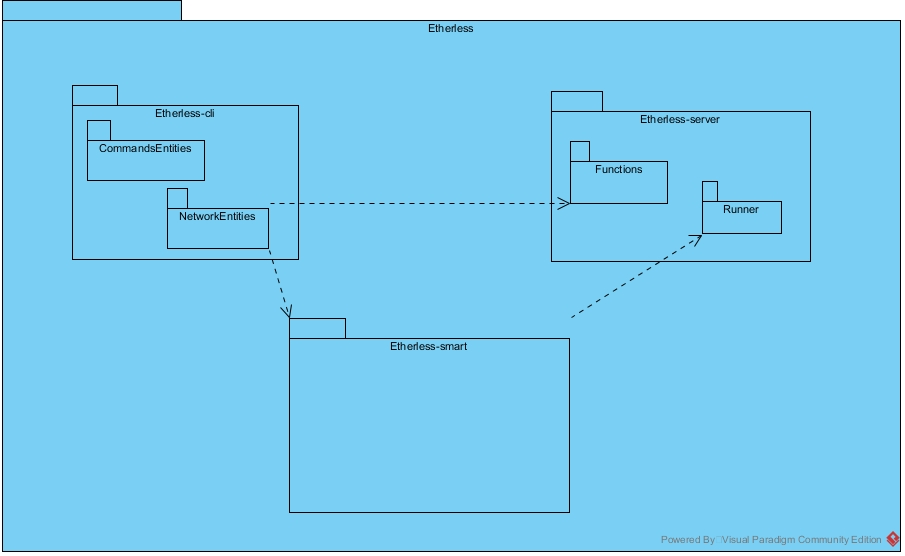
\includegraphics[width=\textwidth]{res/img/packageDiagram.jpg}
	\caption{Package diagram of Ethereum system}
\end{figure}
%In Typescript, the use of packages is not allowed, so the package diagram refers to project folders and its class dependencies.\\
%In the next section are explained all the possible communications between them.
\subsection{Architecture models}
Etherless makes use of multiple architectures. 
\subsubsection{Serverless}
Serverless architecture\glo is a software design pattern where applications are hosted by a third-party service, eliminating the need for server software and hardware management by the developer. Applications are broken up into individual functions that can be invoked and scaled individually.\newline\newline The component etherless-server takes advantage of this architecture with both its modules:
\begin{itemize}
	\item \textbf{Functions:} a set of independent functions that are hosted on AWS as Lambda functions and that serve different Ethereless purposes when called;
	\item \textbf{Runner:} an always running Ethereum\glo network listener ready to take action when trigger events are received; this module is deployed using AWS Elastic Beanstalk, which means that only application code is sent out and server environment is automatically built and managed accordingly based on application requirements;
\end{itemize}
This choice gives us the advantage of not having to worry about server infrastructure or scalability.
Also, JavaScript\glo functions uploaded by users are hosted and run through AWS Lambda which means they too take advantage of all serverless\glo features.
\subsection{Event driven}
This distributed asynchronous architecture consists of single-purpose event processing components that listen on events and process them.\newline
As per requisites, this software design pattern has been used for communication between the three components when a user requests a function execution. The broker topology has been used, as there is not a central events mediator. Events are independent and the smart contract is used as broker as it is the only component that can emit events in the Ethereum network. Event processors are both etherless-cli and etherless-server as they both listen for events at different stages. Check Communication pattern 2 for a more in-depth explanation of events usage.
\newpage
\subsection{Communication}
The communication between these three components is key in understanding the dynamics of the software. We can identify three patterns that can be used based on what the neccesity is.
These three following sequence diagrams are informal and could not satisfy fully UML guidelines.
\subsubsection{Communication pattern 1}
Some functionalities that rely on this communication flow are: functions listing, get function details.
\begin{figure}[h]
	\centering
	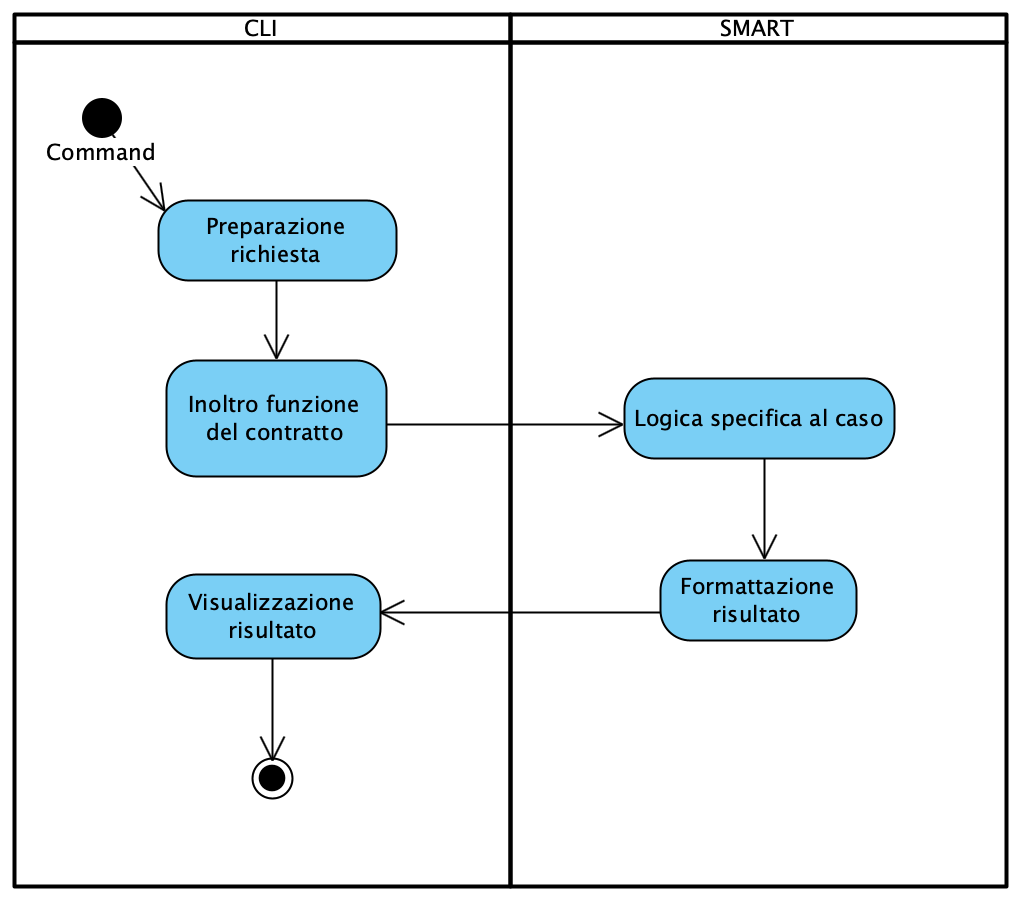
\includegraphics[width=0.8\textwidth]{res/img/pattern1.png}
	\caption{Communication pattern 1 overview}
\end{figure}
\noindent When a user launches a commands that requires the retrivial of information from the smart contract, a contract call is initiated. When the response is received, it gets displayed to the user through the command line window.\newline 
\newpage
\subsubsection{Communication pattern 2}
In some cases the smart component will need to speak directly to the server component. Since smart contracts are unable to perform external calls, the only mean of communication is through Ethereum events. There is a part of etherless-server that is always listening for network events and, once captured, an adeguate response is computed and sent back to the contract (via contract call).\newline Since the communication between the smart and server components is asynchronous , events are used to get back to the cli components as final step.
\begin{figure}[H]
	\centering
	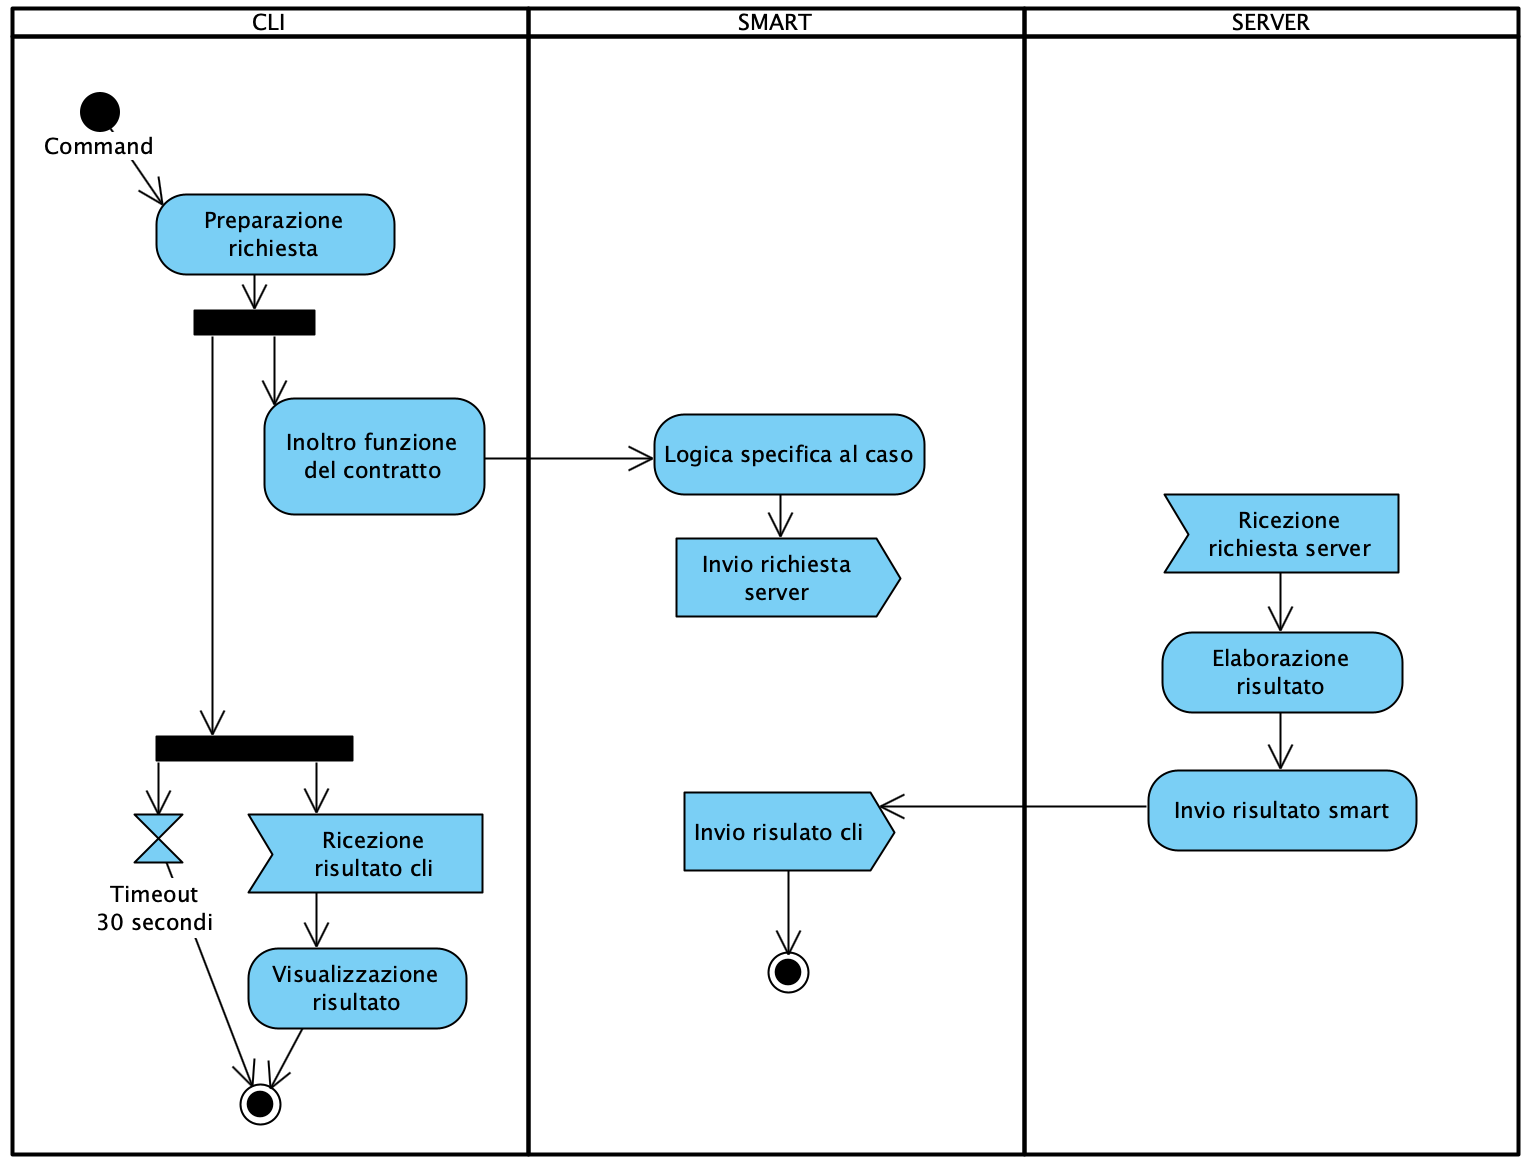
\includegraphics[width=0.8\textwidth]{res/img/pattern2.png}
	\caption{Communication pattern 2 overview}
\end{figure}
Some functionalities that rely on this communication flow are: function creation;
\newpage
\subsubsection{Communication pattern 3}
There might be cases when a resource needs to be deployed to the server component and after getting a successful response, the contract can be updated.
\begin{figure}[H]
	\centering
	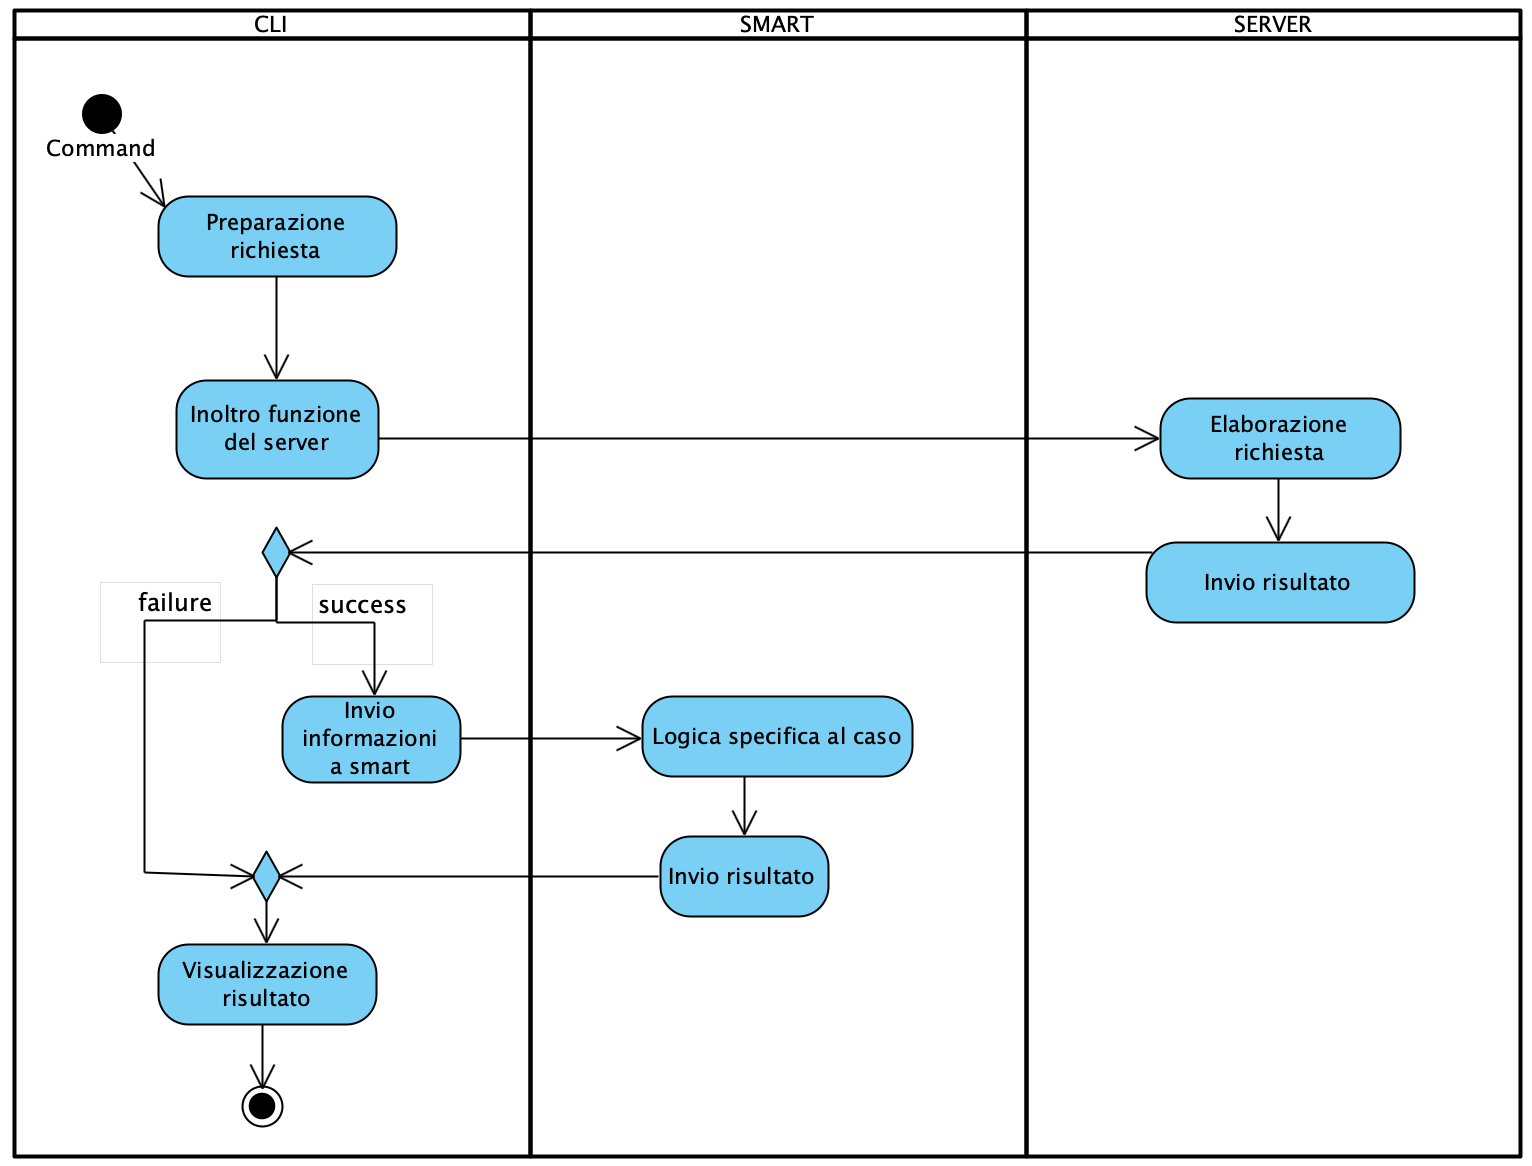
\includegraphics[width=0.8\textwidth]{res/img/pattern3.png}
	\caption{Communication pattern 3 overview}
\end{figure}
Some functionalities that rely on this communication flow are: function remote execution; 